\documentclass{beamer}

%\includeonlyframes{current}
%\includeonly{co}

\usepackage[T1]{fontenc}
\usepackage[utf8]{inputenc}
\usepackage[provide=*,spanish]{babel}
\usepackage{beramono}
\usepackage{hyperref}
\usepackage{graphicx}

\usepackage[dvipsnames]{xcolor}
\definecolor{keyword}{RGB}{0,63,127}
\colorlet{mono}{green!20} %Color para el código monomórfico
\colorlet{poli}{yellow} % Color para el código polimórfico

\usepackage{pgfplots}
\usepackage{tikz}
\usetikzlibrary{positioning,fit,arrows,shapes.arrows,matrix,fit,patterns}
\tikzset{%
  ptr/.style={%
    ->,
    line width=0.3mm
  }
}

\usepackage{listings}
\lstdefinelanguage{java}{
  keywords={
    abstract,
    class,
    extends,
    final, for,
    implements, interface,
    new,
    private, protected, public,
    return,
    this, try,
    var, void,
    while},
  morekeywords={},
  ndkeywords={shapeof},
  sensitive=false,
  comment=[l]{//},
  morecomment=[s]{/*}{*/},
  morestring=[b]',
  morestring=[b]",
  morestring=[b]`,
  morecomment=[l][\color{jsoutput}\bfseries]{<<<}
}
\lstset{
  language=java,
  %backgroundcolor=\color{lightgray},
  basicstyle=\footnotesize\ttfamily,
  emphstyle=\underline,
  keywordstyle=\color{keyword}\bfseries,
  ndkeywordstyle=\color{red}\bfseries,
  identifierstyle=\color{black},
  commentstyle=\color{purple},
  stringstyle=\color{red},
  extendedchars=true,
  showstringspaces=false,
  showspaces=false,
  numbers=left,
  numberstyle=\tiny,
  numbersep=9pt,
  xleftmargin=2em,
  %frame=single,
  framexleftmargin=1.5em,
  tabsize=2,
  breaklines=true,
  showtabs=false,
  captionpos=b
}

% Paquete dentro de https://github.com/MartinScharrer/lstaddons
% Tiene un bug que en mi distro no estaba corregido:
% https://github.com/MartinScharrer/lstaddons/commit/059375e96cdf702cf836c50fcbea920a7aab5752
% Tuve que tocar /usr/share/texmf-dist/tex/latex/lstaddons/lstlinebgrd.sty
\usepackage{lstlinebgrd}


\mode<presentation>{
  %\setbeamertemplate{background canvas}[vertical shading][bottom=red!10,top=blue!10]
  \usetheme{Boadilla}
  \usefonttheme[onlysmall]{structurebold}
}

\title[Stack Allocation]{Stack Allocation\\y otros Monstruos}
\author[Pedro]{
  Pedro Palao Gostanza
}
\institute{Seismo Technologies}
\date{2024-10-30}

\defbeamertemplate*{title page}{customized}[1][]{
  \hbox to\hsize{\hss
    \begin{minipage}{0.5\textwidth}
      {\usebeamerfont{title}\color{RoyalPurple}\bfseries\inserttitle\par}
      \vskip1cm
      \begin{flushright}
      \insertauthor\par
      \insertinstitute\par
      \vskip1cm
      \tiny\insertdate\par
      \end{flushright}
    \end{minipage}
    \hss
    \begin{minipage}{0.5\textwidth}
      \hbox to\textwidth{\hss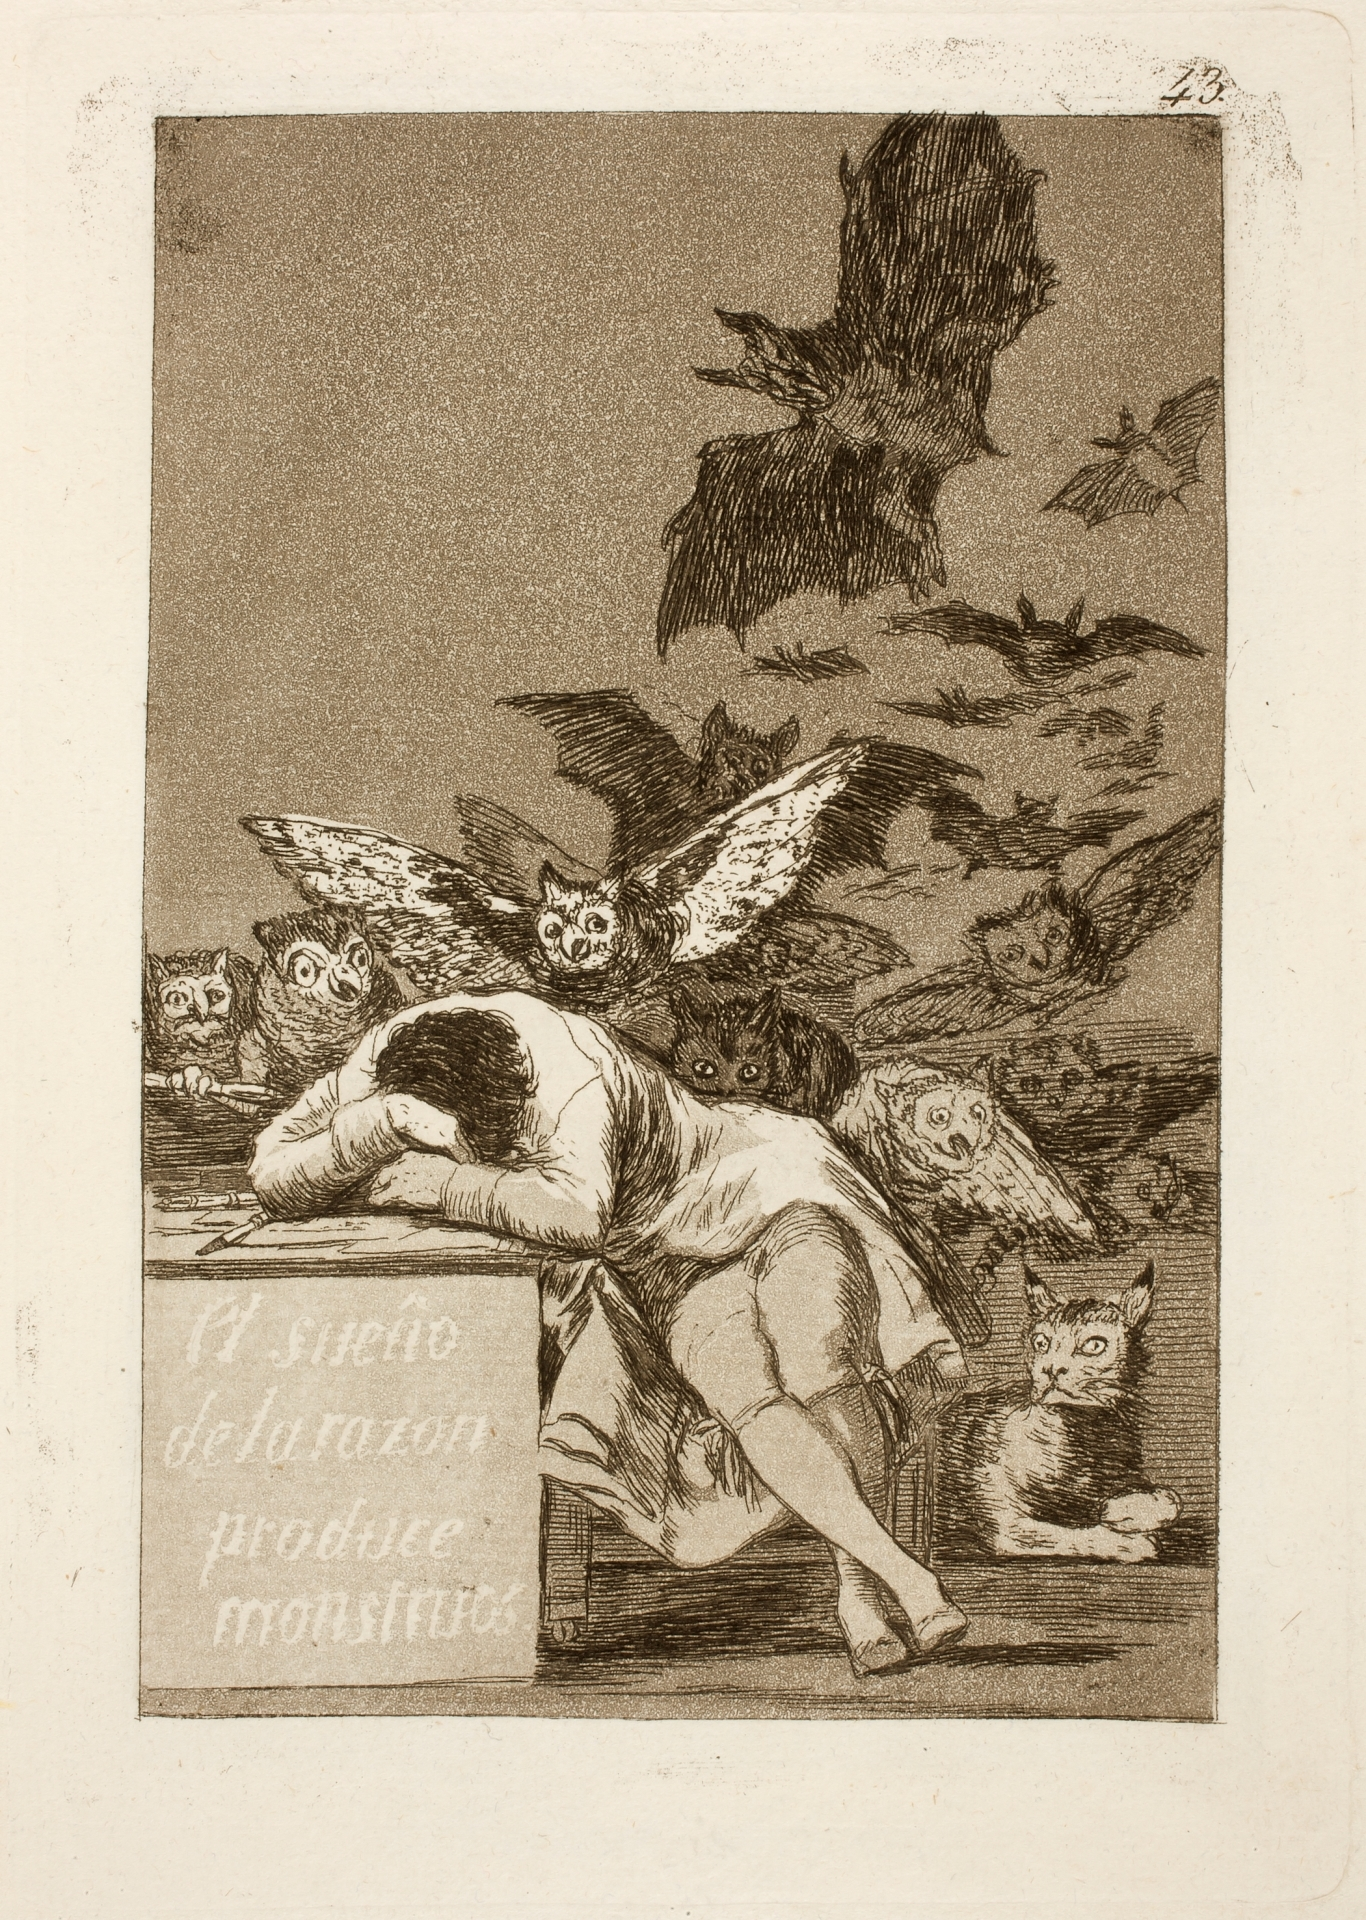
\includegraphics[width=0.8\textwidth]{monstruos.jpg}\hss}%
    \end{minipage}
    \hss}%
}
\begin{document}

\maketitle

\section{Introducción}
% En el título:
% - Voy a hablar de Stack Allocation otros elementos de la java, más bien de
% la jvm, que son relevantes, que tienen una interacción, unas veces positiva
% y otras no tanto, pero veremos cómo soslayar los problemas


\section{Toma de contacto}
\def\ft{Toma de contacto}

% - Antes de empezar con la chicha, 2 puntualizaciones

% - Hay algo de información, no mucha, sobre SA en la red.
% Por una parte, hay información muy técnica, relativa a algoritmos de EA o
% a implementaciones en la JVM.
% Por otra, hay información muy superficial de la operativa de SA o muy
% puntual sobre algún detalle.
% El planteamiento de esta charla es distinto. Nace de la experiencia de
% intentar aprovechar SA en programas o librerías reales para conseguir
% una mejora en el código, simultáneamente en rendimiento y en legibilidad.

% - Y ya que hablamos de rendimiento, una definición somera de SA podría ser
% esta ...
% Por ahora vamos a destacar la palabra *optimización*.
% Si una charla habla de mejoras de rendimiento en la JVM, eso mola,
% porque la gente que trabaja en esas cosas tiene derecho a preocuparse
% por el rendimiento de nuestros programas.
% Pero si una charla habla de cómo mejorar el rendimiento de nuestros
% propios programas, entonces entra en una zona pantanosa,
% y necesita una pequeña introducción expiatoria
% porque en otro caso le arrojarán la famosa frase
% ...

\begin{frame}[fragile]
  \frametitle{\ft}
  \begin{block}{Definición}
    Stack Allocation es una
    \only<1>{optimización}\only<2>{{\bf\color{red} optimización}}
    por la que un objeto creado con {\tt new~C(...)}
    se aloja realmente en la pila
  \end{block}
\end{frame}

\begin{frame}[fragile]
  \frametitle{\ft}
  \begin{block}{Donald Knuth / Tony Hoare}
    \visible<2>{We should forget about small efficiencies, say about 97\% of the time:}
    {\only<2>{\color{gray}}Premature optimization is the root of all evil.}
    \visible<2>{Yet we should not pass up our opportunities in that critical 3\%}
  \end{block}
\end{frame}

\begin{frame}[fragile]
  \frametitle{\ft}
  \begin{block}{Diseñar para}
    \begin{itemize}
    \item Corrección
    \item Mantenimiento
    \item Seguridad
    \item Testeo
    \item $\cdots$
    \visible<2>{\item {\bf Rendimiento}}
    \end{itemize}
  \end{block}
\end{frame}


\section{Stack Allocation}

\def\ft{Conceptos}

\begin{frame}[fragile]
  \frametitle{\ft}
  \begin{block}{Los 3 conceptos fundamentales}
    \begin{itemize}
    \item Escape Analysis
    \item Stack Allocation
    \item Scalar Replacement
    \end{itemize}
  \end{block}
\end{frame}

\begin{frame}[fragile]
  \frametitle{\ft}
  \begin{block}{Ejemplo: hash heap}
    \begin{lstlisting}[language=java]
long hash(byte[] d) {
  var h = new CRC32();
  h.update(d);
  return h.getValue();
}
    \end{lstlisting}
  \end{block}
  \vskip0.5cm
  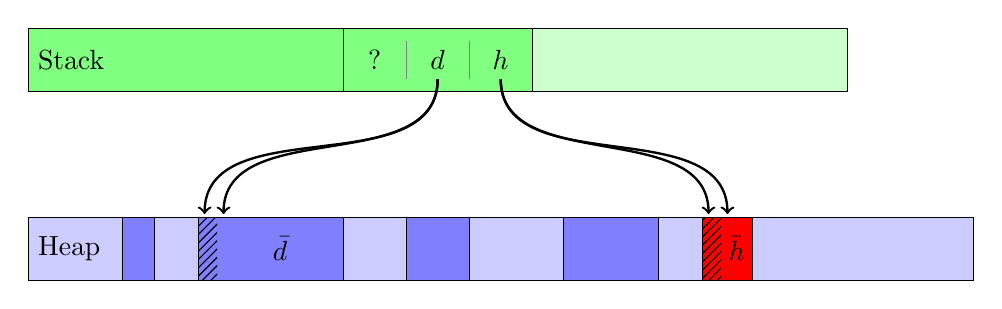
\begin{tikzpicture}[scale=0.8]
    \onslide<2->{\filldraw[draw=black,fill=green!20] (0,3) rectangle +(13,1);}
    \onslide<3->{\filldraw[draw=black,fill=green!50] (0,3) rectangle +(5,1);}
    \onslide<2->{\draw (0,3.5) node[anchor=west] {Stack};}

    \onslide<4-9>{
    \filldraw[draw=black,fill=green!50] (5,3) rectangle +(3,1);
    \draw[draw=black!50]
    (5,3)
    ++(1,0.2) -- ++(0,0.6)
    ++(1,-0.6) -- ++(0,0.6);
    \draw
    (5,3)
    ++(0.5,0.5) node {?}
    ++(1,0) node (d) {$d$}
    ++(1,0) node (h) {$h$};
    }

    \onslide<5->{\filldraw[draw=black,fill=blue!20] (0,0) rectangle +(15,1);}
    \onslide<6->{
      \filldraw[draw=black,fill=blue!50] (1.5,0) rectangle +(0.5,1);
      \filldraw[draw=black,fill=blue!50] (3,0) rectangle +(2,1);
      \filldraw[draw=black,fill=blue!50] (6,0) rectangle +(1,1);
      \filldraw[draw=black,fill=blue!50] (8.5,0) rectangle +(1.5,1);
    }
    \onslide<8>{
      \filldraw[draw=black,fill=blue!50] (11,0) rectangle +(0.5,1);
    }
    \onslide<9->{
      \filldraw[draw=black,fill=blue!50] (2.7,0) rectangle +(2.3,1);
      \fill[pattern={north east lines}] (2.7,0) rectangle +(0.3,1);
      \filldraw[draw=black,fill=blue!50] (10.7,0) rectangle +(0.8,1);
      \fill[pattern={north east lines}] (10.7,0) rectangle +(0.3,1);
    }
    \onslide<10>{
      \filldraw[draw=black,fill=red] (10.7,0) rectangle +(0.8,1);
      \fill[pattern={north east lines}] (10.7,0) rectangle +(0.3,1);
    }
    \onslide<5->{\draw (0,0.5) node[anchor=west] {Heap};}
    
    \onslide<7-8>{\draw[ptr] (d.south) to[out=270,in=90] (3.1,1.05);}
    \onslide<9>{\draw[ptr] (d.south) to[out=270,in=90] (2.8,1.05);}
    \onslide<7-10>{\draw (4,0.5) node {$\bar d$};}
    \onslide<8>{\draw[ptr] (h.south) to[out=270,in=90] (11.1,1.05);}
    \onslide<9>{\draw[ptr] (h.south) to[out=270,in=90] (10.8,1.05);}
    \onslide<8-10>{\draw (11.25,0.5) node {$\bar h$};}
  \end{tikzpicture}
\end{frame}

\begin{frame}[fragile]
  \frametitle{\ft}
  \begin{block}{Escape Analysis}
    \begin{itemize}
    \item Si un objeto solo vive mientras está activa la llamada al método,
      entonces se puede alojar en la pila
    \item Para confirmar que no sobrevive:
      \begin{itemize}
      \item No se devuelve,
      \item No se guarda en otro objeto
      \item Ni en una variable global
      \item ...
      \end{itemize}
      Esto es {\bfseries Escape Analysis {\it Pa'Trás}}
    \end{itemize}
  \end{block}
\end{frame}

\begin{frame}[fragile]
  \frametitle{\ft}
  \begin{block}{Ejemplo: hash stack}
    \begin{lstlisting}[language=java]
long hash(byte[] d) {
  var h = new CRC32();
  h.update(d);
  return h.getValue();
}
    \end{lstlisting}
  \end{block}
  \vskip0cm
  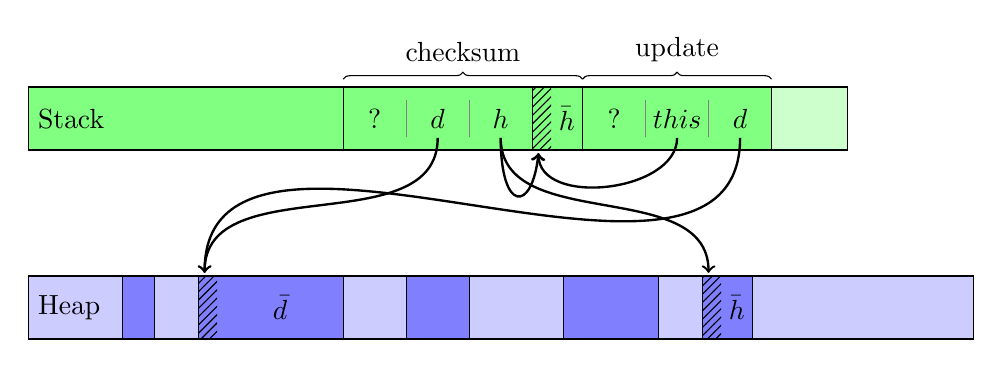
\begin{tikzpicture}[scale=0.8]
    \onslide<1->{\filldraw[draw=black,fill=green!20] (0,3) rectangle +(13,1);}
    \onslide<1->{\filldraw[draw=black,fill=green!50] (0,3) rectangle +(5,1);}
    \onslide<1->{\draw (0,3.5) node[anchor=west] {Stack};}

    \onslide<1->{
    \filldraw[draw=black,fill=green!50] (5,3) rectangle +(3,1);
    \draw[draw=black!50]
    (5,3)
    ++(1,0.2) -- ++(0,0.6)
    ++(1,-0.6) -- ++(0,0.6);
    \draw
    (5,3)
    ++(0.5,0.5) node {?}
    ++(1,0) node (d) {$d$}
    ++(1,0) node (h) {$h$};
    }

    \onslide<1->{\filldraw[draw=black,fill=blue!20] (0,0) rectangle +(15,1);}
    \onslide<1->{
      \filldraw[draw=black,fill=blue!50] (1.5,0) rectangle +(0.5,1);
      \filldraw[draw=black,fill=blue!50] (6,0) rectangle +(1,1);
      \filldraw[draw=black,fill=blue!50] (8.5,0) rectangle +(1.5,1);
    }
    \onslide<1->{
      \filldraw[draw=black,fill=blue!50] (2.7,0) rectangle +(2.3,1);
      \fill[pattern={north east lines}] (2.7,0) rectangle +(0.3,1);
    }
    \onslide<1>{
      \filldraw[draw=black,fill=blue!50] (10.7,0) rectangle +(0.8,1);
      \fill[pattern={north east lines}] (10.7,0) rectangle +(0.3,1);
    }
    \onslide<1->{\draw (0,0.5) node[anchor=west] {Heap};}
    
    \onslide<1->{\draw[ptr] (d.south) to[out=270,in=90] (2.8,1.05);}
    \onslide<1->{\draw (4,0.5) node {$\bar d$};}
    \onslide<1>{\draw[ptr] (h.south) to[out=270,in=90] (10.8,1.05);}
    \onslide<1>{\draw (11.25,0.5) node {$\bar h$};}
    
    \onslide<2->{
      \filldraw[draw=black,fill=green!50] (8,3) rectangle +(0.8,1);
      \fill[pattern={north east lines}] (8,3) rectangle +(0.3,1);
      \draw (8.55,3.5) node {$\bar h$};
      \draw[ptr] (h.south) .. controls (7.5,2) and (8.0,2) .. (8.1,2.95);
    }
    \onslide<3->{
      \draw[decorate,decoration={brace,raise=1mm}]
      (5,4) -- (8.8,4) node[midway,above,yshift=2mm] {checksum};
      
      \filldraw[draw=black,fill=green!50] (8.8,3) rectangle +(3,1);
      \draw[draw=black!50]
      (8.8,3)
      ++(1,0.2) -- ++(0,0.6)
      ++(1,-0.6) -- ++(0,0.6);
      \draw
      (8.8,3)
      ++(0.5,0.5) node {?}
      ++(1,0) node (uthis) {$this$}
      ++(1,0) node (ud) {$d$};
      \draw[decorate,decoration={brace,raise=1mm}]
      (8.8,4) -- (11.8,4) node[midway,above,yshift=2mm] {update};
      \draw[ptr] (uthis) to[out=270,in=270] (8.1,2.95);
      \draw[ptr] (ud) to[out=270,in=90] (2.8,1.05);
    }
  \end{tikzpicture}
\end{frame}

\begin{frame}[fragile]
  \frametitle{\ft}
  \begin{block}{Implicaciones de colocar objetos completos en la pila}
    \begin{itemize}
    \item Exige cambios significativos en GC:
      \begin{itemize}
      \item La búsqueda de raíces en la pila tiene que tratar con objetos
      \item El marcado tiene que tener en cuenta si un objeto está ubicado
        en la pila
      \item El barrido no tiene que eliminar la basura en la pila
      \end{itemize}
    \item Mejora el rendimiento
      \begin{itemize}
      \item Es más sencillo colocar el objeto en la pila
      \item No se genera basura
      \item Hay efectos indirectos: más localidad en los datos
      \end{itemize}
    \item Permite sincronizaciones
    \item Permite {\it escape {\bfseries Pa'Lante}}
    \end{itemize}
  \end{block}
\end{frame}


\begin{frame}[fragile]
  \frametitle{\ft}
  \begin{block}{Monstruo 1: Inlining: la madre de todas las optimizaciones}
    Reemplazar una llamada a un método por su código
  \end{block}
\end{frame}

\begin{frame}[fragile]
  %\frametitle{\ft}
  \begin{block}{Código relevante de CRC32}
    \begin{lstlisting}[language=java]
public interface Checksum {
  default void update(byte[] b) {update(b,0,b.length);}
}
public class CRC32 implements Checksum {
  private int crc = 0;
  
  public long getValue() {return (long)crc & 0xffffffffL;}
  
  public void update(byte[] b, int off, int len) {
    crc = updateBytes(crc, b, off, len);
  }
  static int updateBytes(int crc,
        byte[] b, int off, int len) {
    return updateBytes0(crc, b, off, len);
  }
  @IntrinsicCandidate
  static native int updateBytes0(int crc,
      byte[] b, int off, int len);
}
    \end{lstlisting}
  \end{block}
\end{frame}

\begin{frame}[fragile]
  \frametitle{\ft}
  \begin{block}{Ejecución reiterada del método {\tt hash}}
\begin{lstlisting}
-XX:+UnlockDiagnosticVMOptions
-XX:+PrintCompilation
-XX:+PrintInlining
\end{lstlisting}
\small
\begin{lstlisting}
::hash (22 bytes)   made not entrant
@ 4   CRC32::<init> (5 bytes)   inline (hot)
  @ 1   Object::<init> (1 bytes)   inline (hot)
@ 10   Checksum::update (11 bytes)   inline (hot)
  @ 5   CRC32::update (38 bytes)   inline (hot)
    @ 31   CRC32::updateBytes (14 bytes)   inline (hot)
      @ 10   CRC32::updateBytes0 (0 bytes)   (intrinsic)
@ 16   CRC32::getValue (10 bytes)   inline (hot)
\end{lstlisting}
  \end{block}
\end{frame}

\begin{frame}[fragile]
  \frametitle{\ft}
  \begin{block}{Método {\tt hash} tras hacer inlining}
    \begin{lstlisting}[language=java]
long hash(byte[] d) {
  var h = new Object() {int crc;};
  h.crc = 0;
  h.crc = updateBytes0(h.crc, d, 0, d.length);
  return (long)h.crc & 0xffffffffL;
}
    \end{lstlisting}
  \end{block}
  \vskip1cm
  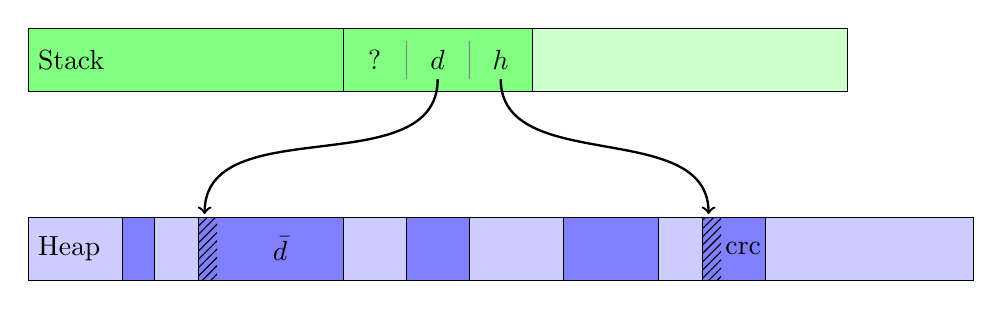
\begin{tikzpicture}[scale=0.8]
    \filldraw[draw=black,fill=green!20] (0,3) rectangle +(13,1);
    \filldraw[draw=black,fill=green!50] (0,3) rectangle +(5,1);
    \draw (0,3.5) node[anchor=west] {Stack};

    \filldraw[draw=black,fill=green!50] (5,3) rectangle +(3,1);
    \draw[draw=black!50]
    (5,3)
    ++(1,0.2) -- ++(0,0.6)
    ++(1,-0.6) -- ++(0,0.6);
    \draw
    (5,3)
    ++(0.5,0.5) node {?}
    ++(1,0) node (d) {$d$}
    ++(1,0) node (h) {$h$};

    \filldraw[draw=black,fill=blue!20] (0,0) rectangle +(15,1);
    \draw (0,0.5) node[anchor=west] {Heap};
    \filldraw[draw=black,fill=blue!50] (1.5,0) rectangle +(0.5,1);
    \filldraw[draw=black,fill=blue!50] (6,0) rectangle +(1,1);
    \filldraw[draw=black,fill=blue!50] (8.5,0) rectangle +(1.5,1);
    
    \filldraw[draw=black,fill=blue!50] (2.7,0) rectangle +(2.3,1);
    \fill[pattern={north east lines}] (2.7,0) rectangle +(0.3,1);
    \draw (4,0.5) node {$\bar d$};
    \draw[ptr] (d.south) to[out=270,in=90] (2.8,1.05);
    
    \filldraw[draw=black,fill=blue!50] (10.7,0) rectangle +(1,1);
    \fill[pattern={north east lines}] (10.7,0) rectangle +(0.3,1);
    \draw (11.35,0.5) node {crc};
    \draw[ptr] (h.south) to[out=270,in=90] (10.8,1.05);    
  \end{tikzpicture}
\end{frame}


\begin{frame}[fragile]
  \frametitle{\ft}
  \begin{block}{Método {\tt hash} tras hacer Scalar Replacement}
    \begin{lstlisting}[language=java]
long hash(byte[] d) {
  int crc = 0;
  crc = updateBytes0(crc, d, 0, d.length);
  return (long)crc & 0xffffffffL;
}
    \end{lstlisting}
  \end{block}
  \vskip1cm
  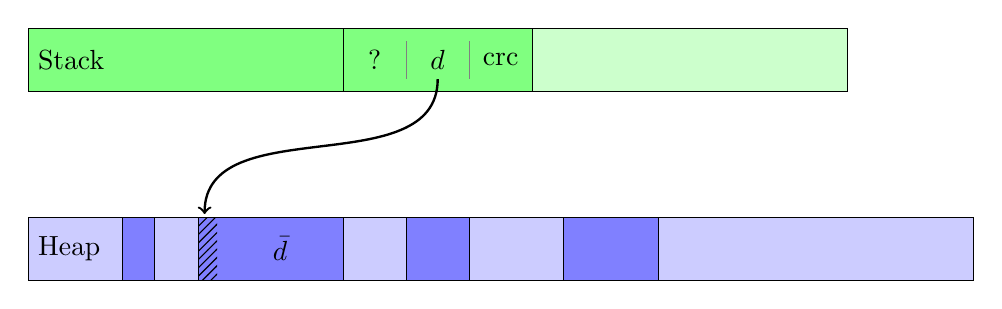
\begin{tikzpicture}[scale=0.8]
    \filldraw[draw=black,fill=green!20] (0,3) rectangle +(13,1);
    \filldraw[draw=black,fill=green!50] (0,3) rectangle +(5,1);
    \draw (0,3.5) node[anchor=west] {Stack};

    \filldraw[draw=black,fill=green!50] (5,3) rectangle +(3,1);
    \draw[draw=black!50]
    (5,3)
    ++(1,0.2) -- ++(0,0.6)
    ++(1,-0.6) -- ++(0,0.6);
    \draw
    (5,3)
    ++(0.5,0.5) node {?}
    ++(1,0) node (d) {$d$}
    ++(1,0) node (h) {crc};

    \filldraw[draw=black,fill=blue!20] (0,0) rectangle +(15,1);
    \draw (0,0.5) node[anchor=west] {Heap};
    \filldraw[draw=black,fill=blue!50] (1.5,0) rectangle +(0.5,1);
    \filldraw[draw=black,fill=blue!50] (6,0) rectangle +(1,1);
    \filldraw[draw=black,fill=blue!50] (8.5,0) rectangle +(1.5,1);
    
    \filldraw[draw=black,fill=blue!50] (2.7,0) rectangle +(2.3,1);
    \fill[pattern={north east lines}] (2.7,0) rectangle +(0.3,1);
    \draw (4,0.5) node {$\bar d$};
    \draw[ptr] (d.south) to[out=270,in=90] (2.8,1.05);    
  \end{tikzpicture}
\end{frame}


\begin{frame}[fragile]
  \frametitle{\ft}
  \begin{block}{Definiciones}
    \begin{itemize}
    \item Escape Analysis: Determina el ambito dinámico de un objeto
    \item Partial Escape Analysis: Variante más sofisticada que es capaz de
      operar sobre bifurcaciones en el código
    \item Stack Allocation: Coloca objetos {\it completos} en la pila.
      Sólo se puede hacer si no sobrevive al método
    \item Scalar Replacement: Coloca los campos de un objeto en la pila.
      Sólo se puede hacer si no escapa del método (en ningún sentido).
      Los campos no tienen por qué estar consecutivos, y podrían limitarse
      a registros del procesador.
      Es un {\it caso especial} de Stack Allocation pero no una {\it mejora}
    \end{itemize}
  \end{block}
\end{frame}


\begin{frame}[fragile]
  \frametitle{\ft}
  \begin{block}{Estado del arte}
    \begin{description}
    \item[C2]
      Escape Analysis,
      Scalar Replacement para objetos
    \item[GraalVM]
      Partial Escape Analysis,
      Scalar Replacement para objetos,
      Scalar replacement limitado para arrays
    \item[OpenJ9]
      Partial Escape Analysis,
      {\bf Stack Allocation} para objetos,
      Scalar Replacement para objetos
    \item[Azul Zing]
      Partial Escape Analysis,
      Scalar Replacement para objetos,
      Scalar replacement limitado para arrays
    \end{description}
  \end{block}
\end{frame}    


\section{Ejemplo: Hashing}

\def\ft{Algoritmos de hashing}

\begin{frame}[fragile]
  \frametitle{\ft}
  \begin{block}{Definición y actores}
    \begin{itemize}
    \item Dado un dato de tamaño arbitrario produce un resumen de N bits
    \item Las garantías del resumen tienen diversos niveles:
      dispersión, dificultad de colisión, uso criptográfico
    \item Multitud de actores con variantes
      CRC32,
      Adler,
      MurmurHash (1, 2 y 3),
      xxHash (XXH32, XXH64, XXH3\_64, XXH3\_128),
      CityHash,
      MetroHash,
      SipHash,
      ...
    \item Siempre trabajan igual
      \begin{itemize}
      \item Descomponen la entrada en bloques de tamaño fijo + una cola
      \item Procesan los bloques secuencialmente
      \item Hay un proceso de cierre, en el que suele intervenir la longitud
        total, y que produce el resumen
      \end{itemize}
    \end{itemize}
  \end{block}
\end{frame}

\begin{frame}[fragile]
  \frametitle{\ft}
  \begin{block}{Planteamientos usuales: hashing para diversos tipos}
    \begin{lstlisting}[language=java]
public interface Hashing {
  long hash(byte x);
  long hash(char x);
  long hash(short x);
  long hash(int x);
  long hash(long x);
  long hash(float x);
  long hash(double x);

  long hash(byte[] xs);
  long hash(byte[] xs, int off, int len);

  long hash(char[] xs);
  long hash(char[] xs, int off, int len);
  long hash(String xs);
  long hash(String xs, int off, int len);
}
    \end{lstlisting}
  \end{block}
\end{frame}

\begin{frame}[fragile]
  \frametitle{\ft}
  \begin{block}{Planteamientos usuales: hashing incremental}
    \begin{lstlisting}[language=java]
public interface Hasher {
  Hasher add(byte x);
  Hasher add(char x);
  Hasher add(short x);
  Hasher add(int x);
  Hasher add(long x);
  Hasher add(float x);
  Hasher add(double x);
  Hasher add(byte[] xs);
  Hasher add(byte[] xs, int off, int len);
  Hasher add(char[] xs);
  Hasher add(char[] xs, int off, int len);
  Hasher add(String xs);
  Hasher add(String xs, int off, int len);

  long hash64();
  int hash(long[] h);
}
    \end{lstlisting}
  \end{block}
\end{frame}

\begin{frame}[fragile]
  \frametitle{\ft}
  \begin{block}{Los {\tt Hasher} se implementan usualmente con un buffer}
    \begin{lstlisting}[language=java]
public class AbstractHasher implements Hasher {
  private byte[] buf;
  private int used;

  protected AbstractHasher() {
    this.buf = new byte[BLOCK_SIZE+7];
    this.used = 0;
  }
  ...
  public Hasher add(int x) {
    Bits.le32(buf, used, x);
    used += 4;
    mayFlush();
    return this;
  }
  ...
}
    \end{lstlisting}
  \end{block}
\end{frame}


\begin{frame}[fragile]
  \frametitle{\ft}
  \begin{block}{¿Cómo se implementa un {\tt Hashing}?}
    \begin{itemize}
    \item A través de un Hasher, salvo para {\tt byte[]}
      (\href{https://github.com/google/guava/blob/master/guava/src/com/google/common/hash/AbstractHashFunction.java}{Guava})
    \item Especializando el código del algoritmo a mano para cada tipo
      (\href{https://github.com/OpenHFT/Zero-Allocation-Hashing/blob/ea/src/main/java/net/openhft/hashing/XxHash.java}{Zero-Allocation-Hashing})
    \end{itemize}
  \end{block}
\end{frame}


\begin{frame}[fragile]
  \frametitle{\ft}
  \begin{block}{Hashish: el experimento fumeta}
    \begin{itemize}
    \item Hashish es una librería de hashing que intenta congujar
      (1) un diseño con descomposición de responsabilidades
      con (2) el mejor rendimiento posible en Java
    \item Para ello se basa fuertemente en Scalar Replacement
    \item Introduce el concepto de {\tt Kernel}
    \end{itemize}
  \end{block}
\end{frame}


\begin{frame}[fragile]
  \frametitle{\ft}
  \begin{block}{Hashish: Un kernel para cada tamaño de bloque}
    \begin{lstlisting}[language=java]
public interface Kernel64 {
  void block(long block);
  void tail(long tail, int taillen, long total);
}

public interface Kernel128 {
  void block(long b0, long b1);
  void tail(long b0, long b1, int taillen, long total);
}
    \end{lstlisting}
  \end{block}
\end{frame}


\begin{frame}[fragile]
  \frametitle{\ft}
  \begin{block}{Hashish: Los kernels se crean a cascoporro}
    \begin{lstlisting}[language=java]
public abstract class HashingKernel64 implements Hashing {
  protected abstract Kernel64 newKernel();
  public long hash(byte x) {
    return integral(Bits.ubyte(x), 1);
  }
  ...
  private long integral(long x, int taillen) {
    Kernel64 kernel = newKernel();
    kernel.tail(x, taillen, taillen);
    return kernel.hash();
  }
  public long hash(long x) {
    Kernel64 kernel = newKernel();
    kernel.block(x);
    kernel.tail(0, 0, 8);
    return kernel.hash();
  }
  ...
    \end{lstlisting}
  \end{block}
\end{frame}


\begin{frame}[fragile]
  \frametitle{\ft}
  \begin{block}{Hashish: Los kernels se crean a cascoporro 2}
    \begin{lstlisting}[language=java]
  ...

  public long hash(byte[] xs, int off, int len) {
    final int W = 8;
    final Kernel64 kernel = newKernel();
    final int blockno = len / W;
    for (int i = 0; i < blockno; i++) {
      kernel.block(Bits.le64(xs, off + W*i));
    }
    final int taillen = len - W*blockno;
    kernel.tail(Bits.le64tail(xs, off + W*blockno, taillen), taillen, len);
    return kernel.hash();
  }
}
    \end{lstlisting}
  \end{block}
\end{frame}


\begin{frame}[fragile]
  \frametitle{\ft}
  \begin{block}{Hashish: Para un nuevo algoritmo basta un nuevo Kernel}
    \begin{lstlisting}[language=java]
public class SipHashKernel implements Kernel64 {
  private long v0, v1, v2, v3;

  public void block(long block) {
    v3 ^= block;
    compressionRounds();
    v0 ^= block;
  }

  public void tail(long tail, int taillen, long totallen) {
    final long mask = ~((~0L) << (8*taillen));
    block((mask & tail) | ((totallen & 0xFF) << 56));
    v2 ^= 0xFF;
    finalizationRounds();
  }
  ...
}
    \end{lstlisting}
  \end{block}
\end{frame}


\begin{frame}[fragile]
  \frametitle{\ft}
  \begin{block}{Hashish: ... y definir el Hashing}
    \begin{lstlisting}[language=java]
public class SipHashing extends HashingKernel64 {
  private final long k0, k1;

  public SipHashing(long k0, long k1) {
    this.k0 = k0;
    this.k1 = k1;
  }

  protected SipHashKernel newKernel() {
    return new SipHashKernel(k0,k1);
  }
}
    \end{lstlisting}
  \end{block}
\end{frame}


\begin{frame}[fragile]
  \frametitle{\ft}
  \begin{block}{Rendimiento sobre byte[3]}
    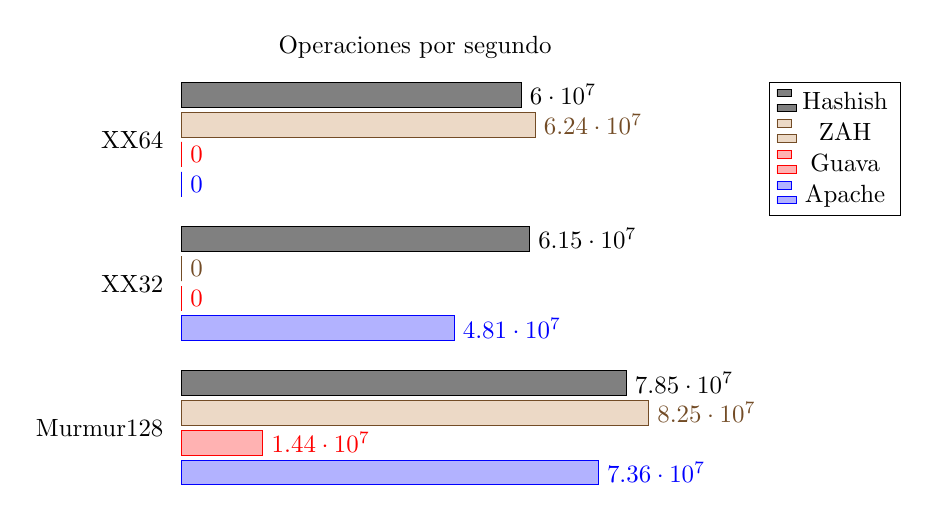
\begin{tikzpicture}[scale=0.9]
      \begin{axis}[
          title  = Operaciones por segundo,
          xbar,
          xmin=0,
          y axis line style = { opacity = 0 },
          axis x line       = none,
          tickwidth         = 0pt,
          enlarge y limits  = 0.2,
          enlarge x limits  = 0.02,
          symbolic y coords = {Murmur128, XX32, XX64},
          ytick=data,
          nodes near coords,
          reverse legend,
          %legend pos=north east,
          legend style={at={(1.5,1)}, anchor=north east},
        ]
        % apache
        \addplot coordinates {
          (73589373.939,Murmur128)
          (48119911.412,XX32)
          (0,XX64)
        };
        % guava
        \addplot coordinates {
          (14371913.397,Murmur128)
          (0,XX32)
          (0,XX64)
        };
        % ZAH
        \addplot coordinates {
          (82480222.390,Murmur128)
          (0,XX32)
          (62431785.506,XX64)
        };
        % Hashish
        \addplot coordinates {
          (78525118.804,Murmur128)
          (61452279.610,XX32)
          (59960144.582,XX64)
        };
        \legend{Apache, Guava, ZAH, Hashish}
      \end{axis}
    \end{tikzpicture}
  \end{block}
\end{frame}


\begin{frame}[fragile]
  \frametitle{\ft}
  \begin{block}{Rendimiento sobre byte[31]}
    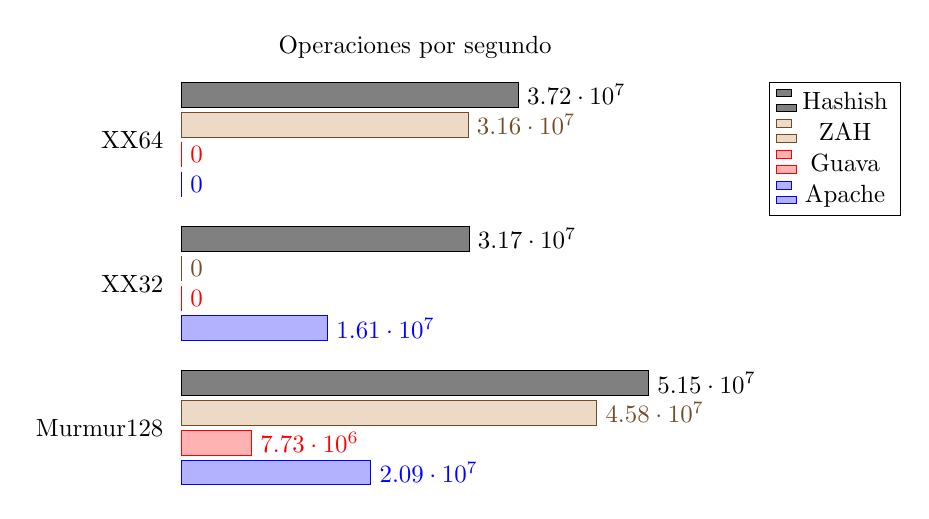
\begin{tikzpicture}[scale=0.9]
      \begin{axis}[
          title  = Operaciones por segundo,
          xbar,
          xmin=0,
          y axis line style = { opacity = 0 },
          axis x line       = none,
          tickwidth         = 0pt,
          enlarge y limits  = 0.2,
          enlarge x limits  = 0.02,
          symbolic y coords = {Murmur128, XX32, XX64},
          ytick=data,
          nodes near coords,
          reverse legend,
          %legend pos=north east,
          legend style={at={(1.5,1)}, anchor=north east},
        ]
        % apache
        \addplot coordinates {
          (20866076.290,Murmur128)
          (16107110.585,XX32)
          (0,XX64)
        };
        % guava
        \addplot coordinates {
          (7734910.459,Murmur128)
          (0,XX32)
          (0,XX64)
        };
        % ZAH
        \addplot coordinates {
          (45790062.374,Murmur128)
          (0,XX32)
          (31611002.009,XX64)
        };
        % Hashish
        \addplot coordinates {
          (51503941.311,Murmur128)
          (31723083.396,XX32)
          (37151254.934,XX64)
        };
        \legend{Apache, Guava, ZAH, Hashish}
      \end{axis}
    \end{tikzpicture}
  \end{block}
\end{frame}


\begin{frame}[fragile]
  \frametitle{\ft}
  \begin{block}{Rendimiento sobre byte[1048607]}
    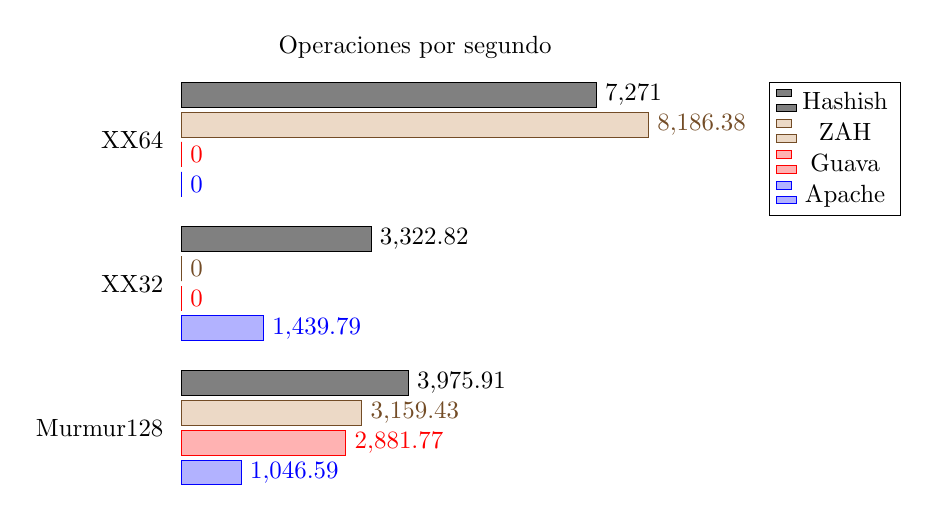
\begin{tikzpicture}[scale=0.9]
      \begin{axis}[
          title  = Operaciones por segundo,
          xbar,
          xmin=0,
          y axis line style = { opacity = 0 },
          axis x line       = none,
          tickwidth         = 0pt,
          enlarge y limits  = 0.2,
          enlarge x limits  = 0.02,
          symbolic y coords = {Murmur128, XX32, XX64},
          ytick=data,
          nodes near coords,
          reverse legend,
          %legend pos=north east,
          legend style={at={(1.5,1)}, anchor=north east},
        ]
        % apache
        \addplot coordinates {
          (1046.593,Murmur128)
          (1439.794,XX32)
          (0,XX64)
        };
        % guava
        \addplot coordinates {
          (2881.766,Murmur128)
          (0,XX32)
          (0,XX64)
        };
        % ZAH
        \addplot coordinates {
          (3159.433,Murmur128)
          (0,XX32)
          (8186.380,XX64)
        };
        % Hashish
        \addplot coordinates {
          (3975.910,Murmur128)
          (3322.824,XX32)
          (7271.002,XX64)
        };
        \legend{Apache, Guava, ZAH, Hashish}
      \end{axis}
    \end{tikzpicture}
  \end{block}
\end{frame}


\section{Testing de Scalar Replacement}

\def\ft{Testing de Scalar Replacement}

\begin{frame}[fragile]
  \frametitle{\ft}
  \begin{block}{Dudas}
    \begin{itemize}
    \item ¿Cómo comprobar si la JVM descubre lo que {\it claramente nos parece}
      un candidato a scalar replacement?
    \item ¿Deberíamos testear scalar replacemente?
    \item ¿Deberíamos testear el rendimiento?
    \item ¿Y ser capaces de detectar regresiones de rendimiento?
    \item Scalar replacement es una optimización tachada de {\it esquiva}
      que además depende de inlining que es {\it incierta}
    \item JMH + inspección visual, de OPS o de GC
    \end{itemize}
  \end{block}
\end{frame}

\begin{frame}[fragile]
  \frametitle{\ft}
  \begin{block}{Objetivo}
    Poder escribir un test (unitario) que compruebe
    que una sección de código no crea objetos de un juego de clases
    \onslide<2->{\color{red}(posiblemente tras unas cuantas iteraciones)}
  \end{block}
\end{frame}


\begin{frame}[fragile]
  \frametitle{\ft}
  \begin{block}{Posible idea: estadísticas de memoria usada}
    \begin{itemize}
    \item {\tt MemoryMXBean.getHeapMemoryUsage()}
      da la cantidad de memoria usada en el heap
    \item {\tt GarbageCollectorMXBean.getCollectionCount()}
      da la cantidad de GCs que ha habido
    \item Combinando ambas podemos ejecutar una sección de código
      y comprobar que (1) no hubo GC y (2) cómo aumentó la memoria
    \item Inconveniente:
      No permite distiguir qué objetos se han creado. Sólo es útil
      si nuestro objeto es el dominante
    \item Descarte:
      los datos de consumo de memoria no se actualizan inmediatamente
    \end{itemize}
  \end{block}
\end{frame}


\begin{frame}[fragile]
  \frametitle{\ft}
  \begin{block}{Posible idea: listener de GC}
    \begin{itemize}
    \item {\tt GarbageCollectorMXBean.addNotificationListener()}
      permite escuchar el resultado de cada GC
    \item {\tt MemoryMXBean.gc()} fuerza un GC
    \item Combinando ambas se puede hacer una limpieza
      (forzar un GC y escuchar la información de su fin),
      ejecutar nuestra sección de código,
      volver a hacer una limpieza.
      La basura de la segunda limpieza la habrá creado nuestra sección de código
    \item Inconveniente:
      No permite distiguir qué objetos se han creado. Sólo es útil
      si nuestro objeto es el dominante
    \item Descarte:
      la propia medida genera basura, en cantidad que depende mucho del
      algoritmo de GC
    \end{itemize}
  \end{block}
\end{frame}


\begin{frame}[fragile]
  \frametitle{\ft}
  \begin{block}{Posible idea: Monstruo 2: hprof}
    \begin{itemize}
    \item {\tt HotSpotDiagnosticMXBean.dumpHeap} permite hacer un volcado
      de la memoria en formato hprof
    \item {\tt HeapFactory.createHeap} de NetBeans
      permite analizar un hprof
    \item Combinadas dan lugar al siguiente esquema
      \begin{enumerate}
      \item Forzamos GC
      \item Hacemos volcado inicial,
        contamos el número $I_c$ de instancias de las clases que nos interesan
        y descartamos el volcado
      \item Ejecutamos nuestra sección de código
      \item Hacemos volcado final
      \item Comprobamos que no ha habido ningún GC
      \item Contamos en el volcado final el número $F_c$ de instancias de las
        clases que nos interesan
      \item $F_c - I_c$ son las instancias creadas
      \end{enumerate}
    \end{itemize}
  \end{block}
\end{frame}


\begin{frame}[fragile]
  %\frametitle{\ft}
  \begin{block}{CRC32: ejemplo de testing}
    \begin{lstlisting}[language=java]
@Test void crc32EventuallyDoesNotAllocate() {
  final byte[] data = new byte[2*4];
  var chk = new TryAllocationChecker(CRC32.class).verbose();
  for (int i = 0; i < 25 && !chk.satisfied(); i++) {
    Bits.le32(data, 0, i);
    try (var ignored = chk.enter()) {
      for (int j = 0; j < 10_000; j++) {
        Bits.le32(data, 4, j);
        chk.consume(crc32(data));
      }
    }
  }
  chk.assertSatisfied();
}
long crc32(byte[] data) {
  var her = new CRC32();
  her.update(data);
  return her.getValue();
}
    \end{lstlisting}
  \end{block}
\end{frame}

\begin{frame}[fragile]
  \frametitle{\ft}
  \begin{block}{CRC32: ejecución testing}
    \begin{lstlisting}
AllocationCheckerTest > crc32EventuallyDoesNotAllocate()
  Allocation: [gcs: 0, instances: CRC32=10066]
  Allocation: [gcs: 0, instances: CRC32=0]
  Allocation: [gcs: 0, instances: CRC32=0]
  Allocation: [gcs: 0, instances: CRC32=0]
  Reduced: 85899345900000
    \end{lstlisting}
  \end{block}
\end{frame}


\begin{frame}[fragile]
  \frametitle{\ft}
  \begin{block}{String concat: ejemplo de testing}
    \begin{lstlisting}[language=java]
@Test void concatEventuallyDoesNotAllocateStringBuilder() {
  var chk = new TryAllocationChecker(StringBuilder.class);
  for (int i = 0; i < 25 && !chk.satisfied(); i++) {
    try (var ignored = chk.enter()) {
      for (int j = 0; j < 10_000; j++) {
        chr.consume(message(i,j));
      }
    }
  }
  chk.assertSatisfied();
}

int message(int i, int j) {
  return ("Esos " + i + " tipos con bigote tienen cara de "
      + j + " otentotes").length();
}
    \end{lstlisting}
  \end{block}
\end{frame}

\begin{frame}[fragile]
  \frametitle{\ft}
  \begin{block}{String concat: ejecución testing}
    \begin{lstlisting}
AllocationCheckerTest > concatEventuallyDoesNotAllocateStringBuilder()
  Allocation: [gcs: 0, instances: StringBuilder=682]
  Allocation: [gcs: 0, instances: StringBuilder=13]
  Allocation: [gcs: 0, instances: StringBuilder=13]
  Allocation: [gcs: 0, instances: StringBuilder=12]
  Reduced: 2155560
    \end{lstlisting}
  \end{block}
\end{frame}


\begin{frame}[fragile]
  \frametitle{\ft}
  \begin{block}{StringBuilder: ejemplo de testing}
    \begin{lstlisting}[language=java]
int message(int i, int j) {
  return new StringBuilder()
    .append("Esos ")
    .append(i)
    .append(" tipos con bigote tienen cara de ")
    .append(j)
    .append(" otentotes")
    .toString()
    .length();
}
    \end{lstlisting}
  \end{block}
\end{frame}

\begin{frame}[fragile]
  \frametitle{\ft}
  \begin{block}{String concat: ejecución testing}
    \begin{lstlisting}
AllocationCheckerTest > concatEventuallyDoesNotAllocateStringBuilder()
  Allocation: [gcs: 0, instances: StringBuilder=10634]
  Allocation: [gcs: 0, instances: StringBuilder=13]
  Allocation: [gcs: 0, instances: StringBuilder=12]
  Allocation: [gcs: 0, instances: StringBuilder=12]
  Reduced: 2155560
    \end{lstlisting}
  \end{block}
\end{frame}


\section{Efecto del polimorfismo}

\def\ft{Efecto del polimorfismo}

\begin{frame}[fragile]
  \frametitle{\ft}
  \begin{block}{Monstruo 3: el polimorfismo}
    \begin{itemize}
    \item Un {\it call site} es un punto de llamada a un método
    \item Se clasifican en monomórficos, polimórficos y megamórficos
      en función de la variedad de clases que son destino de esa llamada
    \item El inlining está limitado por el polimorfismo
    \item Y el scalar replacement está limitado por el inlining
    \item Y ... los métodos heredados no cambian de clase
    \end{itemize}
  \end{block}
\end{frame}


\begin{frame}[fragile]
  \frametitle{\ft}
  \begin{block}{Clase abstracta}
    \begin{lstlisting}[
        language=java,
        linebackgroundcolor={
          \ifnum\value{lstnumber}=6\color{poli}\fi
          \ifnum\value{lstnumber}=7\color{poli}\fi
          \ifnum\value{lstnumber}=8\color{poli}\fi
        }
      ]
public abstract class HashingKernel64 implements Hashing {
  protected abstract Kernel64 newKernel();
  ...
  public long hash(long x) {
    final Kernel64 kernel = newKernel();
    kernel.block(x);
    kernel.tail(0, 0, 8);
    return kernel.hash();
  }
  ...
}
    \end{lstlisting}
  \end{block}
\end{frame}


\begin{frame}[fragile]
  \frametitle{\ft}
  \begin{block}{Uso monomórfico (2)}
    \begin{lstlisting}[
        language=java,
        linebackgroundcolor={
          \ifnum\value{lstnumber}=6\color{mono}\fi
          \ifnum\value{lstnumber}=7\color{mono}\fi
        }
      ]
static final Hashing H1 = new MyHashing1();
static final Hashing H2 = new MyHashing2();

long ultrahash2(long d) {
  return
    H1.hash(d)
    + H2.hash(d);
}
    \end{lstlisting}
  \end{block}
\end{frame}


\begin{frame}[fragile]
  \frametitle{\ft}
  \begin{block}{Clase abstracta: inlining (2)}
    \begin{lstlisting}[basicstyle=\tiny]
HashingKernel64::hash (30 bytes)   made not entrant
@ 1   MyHashing2::newKernel (8 bytes)   inline (hot)
@ 1   MyHashing1::newKernel (8 bytes)   inline (hot)
 \-> TypeProfile (8702/17405 counts) = MyHashing1
 \-> TypeProfile (8703/17405 counts) = MyHashing2
  @ 4   MyKernel1::<init> (6 bytes)   inline (hot)
    @ 2   MyKernel1::<init> (15 bytes)   inline (hot)
      @ 1   java.lang.Object::<init> (1 bytes)   inline (hot)
  @ 4   MyKernel2::<init> (6 bytes)   inline (hot)
    @ 2   MyKernel2::<init> (15 bytes)   inline (hot)
      @ 1   java.lang.Object::<init> (1 bytes)   inline (hot)
@ 7   MyKernel2::block (11 bytes)   inline (hot)
@ 7   MyKernel1::block (11 bytes)   inline (hot)
 \-> TypeProfile (8702/17405 counts) = MyKernel1
 \-> TypeProfile (8703/17405 counts) = MyKernel2
@ 18   MyKernel2::tail (14 bytes)   inline (hot)
@ 18   MyKernel1::tail (14 bytes)   inline (hot)
 \-> TypeProfile (8702/17405 counts) = MyKernel1
 \-> TypeProfile (8703/17405 counts) = MyKernel2
@ 24   MyKernel2::hash (5 bytes)   accessor
@ 24   MyKernel1::hash (5 bytes)   accessor
 \-> TypeProfile (8702/17405 counts) = MyKernel1
 \-> TypeProfile (8703/17405 counts) = MyKernel2
    \end{lstlisting}
  \end{block}
\end{frame}


\begin{frame}[fragile]
  %\frametitle{\ft}
  \begin{block}{Uso monomórfico: inlining (2)}
    \begin{lstlisting}[basicstyle=\tiny]
ultrahash2 @ 54 (147 bytes)   made not entrant
@ 75   HashingKernel64::hash (30 bytes)   inline (hot)
  @ 1   MyHashing1::newKernel (8 bytes)   inline (hot)
    ...
  @ 7   MyKernel2::block (11 bytes)   inline (hot)
  @ 7   MyKernel1::block (11 bytes)   inline (hot)
   \-> TypeProfile (13620/27241 counts) = MyKernel1
   \-> TypeProfile (13621/27241 counts) = MyKernel2
  @ 18   MyKernel2::tail (14 bytes)   inline (hot)
  @ 18   MyKernel1::tail (14 bytes)   inline (hot)
   \-> TypeProfile (13620/27241 counts) = MyKernel1
   \-> TypeProfile (13621/27241 counts) = MyKernel2
  @ 24   MyKernel2::hash64 (5 bytes)   accessor
  @ 24   MyKernel1::hash64 (5 bytes)   accessor
   \-> TypeProfile (13620/27241 counts) = MyKernel1
   \-> TypeProfile (13621/27241 counts) = MyKernel2
@ 85   HashingKernel64::hash (30 bytes)   inline (hot)
  @ 1   MyHashing2::newKernel (8 bytes)   inline (hot)
    ...
  @ 7   MyKernel2::block (11 bytes)   inline (hot)
  @ 7   MyKernel1::block (11 bytes)   inline (hot)
   \-> TypeProfile (13620/27241 counts) = MyKernel1
   \-> TypeProfile (13621/27241 counts) = MyKernel2
  @ 18   MyKernel2::tail (14 bytes)   inline (hot)
  @ 18   MyKernel1::tail (14 bytes)   inline (hot)
   \-> TypeProfile (13620/27241 counts) = MyKernel1
   \-> TypeProfile (13621/27241 counts) = MyKernel2
  @ 24   MyKernel2::hash64 (5 bytes)   accessor
  @ 24   MyKernel1::hash64 (5 bytes)   accessor
   \-> TypeProfile (13620/27241 counts) = MyKernel1
   \-> TypeProfile (13621/27241 counts) = MyKernel2
    \end{lstlisting}
  \end{block}
\end{frame}


\begin{frame}[fragile]
  \frametitle{\ft}
  \begin{block}{Uso monomórfico (3)}
    \begin{lstlisting}[
        language=java,
        linebackgroundcolor={
          \ifnum\value{lstnumber}=7\color{mono}\fi
          \ifnum\value{lstnumber}=8\color{mono}\fi
          \ifnum\value{lstnumber}=9\color{mono}\fi
        }
      ]
static final Hashing H1 = new MyHashing1();
static final Hashing H2 = new MyHashing2();
static final Hashing H3 = new MyHashing3();

long ultrahash3(long d) {
  return
    H1.hash(d)
    + H2.hash(d)
    + H3.hash(d);
}
    \end{lstlisting}
  \end{block}
\end{frame}


\begin{frame}[fragile]
  \frametitle{\ft}
  \begin{block}{Clase abstracta: inlining (3)}
    \begin{lstlisting}[basicstyle=\tiny]
HashingKernel64::hash (30 bytes)   made not entrant
@ 1   HashingKernel64::newKernel (0 bytes)   failed to inline: virtual call
@ 7   Kernel64::block (0 bytes)   failed to inline: virtual call
@ 18   Kernel64::tail (0 bytes)   failed to inline: virtual call
@ 24   Hash::hash64 (10 bytes)   failed to inline: virtual call
    \end{lstlisting}
  \end{block}
\end{frame}


\begin{frame}[fragile]
  \frametitle{\ft}
  \begin{block}{Uso monomórfico: inlining (3)}
    \begin{lstlisting}[basicstyle=\tiny]
ultrahash3 @ 54 (158 bytes)   made not entrant
@ 75   HashingKernel64::hash (30 bytes)   inline (hot)
  @ 1   MyHashing1::newKernel (8 bytes)   inline (hot)
    @ 4   MyKernel1::<init> (6 bytes)   inline (hot)
      @ 2   MyKernel1::<init> (15 bytes)   inline (hot)
        @ 1   java.lang.Object::<init> (1 bytes)   inline (hot)
  @ 7   Kernel64::block (0 bytes)   virtual call
  @ 18   Kernel64::tail (0 bytes)   virtual call
  @ 24   Hash::hash64 (10 bytes)   virtual call
@ 85   HashingKernel64::hash (30 bytes)   inline (hot)
  @ 1   MyHashing2::newKernel (8 bytes)   inline (hot)
    @ 4   MyKernel2::<init> (6 bytes)   inline (hot)
      @ 2   MyKernel2::<init> (15 bytes)   inline (hot)
        @ 1   java.lang.Object::<init> (1 bytes)   inline (hot)
  @ 7   Kernel64::block (0 bytes)   virtual call
  @ 18   Kernel64::tail (0 bytes)   virtual call
  @ 24   Hash::hash64 (10 bytes)   virtual call
@ 96   HashingKernel64::hash (30 bytes)   inline (hot)
  @ 1   MyHashing3::newKernel (8 bytes)   inline (hot)
    @ 4   MyKernel3::<init> (6 bytes)   inline (hot)
      @ 2   MyKernel3::<init> (15 bytes)   inline (hot)
        @ 1   java.lang.Object::<init> (1 bytes)   inline (hot)
  @ 7   Kernel64::block (0 bytes)   virtual call
  @ 18   Kernel64::tail (0 bytes)   virtual call
  @ 24   Hash::hash64 (10 bytes)   virtual call
    \end{lstlisting}
  \end{block}
\end{frame}


\begin{frame}[fragile]
  \frametitle{\ft}
  \begin{block}{Monstruo 4: el splitting}
    \begin{itemize}
    \item Splitting: Intenta eliminar los puntos polimórficos buscando
      un punto de llamada anterior monomórfico
    \item ¿Lo tiene alguna JVM?
    \item Pero un inlining {\it más precavido} tiene un efecto similar
    \end{itemize}
  \end{block}
\end{frame}


\begin{frame}[fragile]
  \frametitle{\ft}
  \begin{block}{Uso monomórfico: C2 v21 al rescate (2)}
    \begin{lstlisting}[basicstyle=\tiny]
ultrahash2 @ 54 (147 bytes)   made not entrant
@ 75   HashingKernel64::hash (30 bytes)   inline (hot)
  @ 1   MyHashing2::newKernel (8 bytes)   inline (hot)
    @ 4   MyKernel1::<init> (6 bytes)   inline (hot)
      @ 2   MyKernel1::<init> (15 bytes)   inline (hot)
        @ 1   java.lang.Object::<init> (1 bytes)   inline (hot)
  @ 7   MyKernel1::block (11 bytes)   inline (hot)
  @ 18   MyKernel1::tail (14 bytes)   inline (hot)
  @ 24   MyKernel1::hash64 (5 bytes)   accessor
@ 85   HashingKernel64::hash (30 bytes)   inline (hot)
  @ 1   MyHashing2::newKernel (8 bytes)   inline (hot)
    @ 4   MyKernel2::<init> (6 bytes)   inline (hot)
      @ 2   MyKernel2::<init> (15 bytes)   inline (hot)
        @ 1   java.lang.Object::<init> (1 bytes)   inline (hot)
  @ 7   MyKernel2::block (11 bytes)   inline (hot)
  @ 18   MyKernel2::tail (14 bytes)   inline (hot)
  @ 24   MyKernel2::hash64 (5 bytes)   accessor
    \end{lstlisting}
  \end{block}
\end{frame}


\begin{frame}[fragile]
  \frametitle{\ft}
  \begin{block}{Uso monomórfico: C2 v21 al rescate (3)}
    \begin{lstlisting}[basicstyle=\tiny]
ultrahash3 @ 54 (158 bytes)   made not entrant
@ 75   HashingKernel64::hash (30 bytes)   inline (hot)
  @ 1   MyHashing3::newKernel (8 bytes)   inline (hot)
    @ 4   MyKernel1::<init> (6 bytes)   inline (hot)
      @ 2   MyKernel1::<init> (15 bytes)   inline (hot)
        @ 1   java.lang.Object::<init> (1 bytes)   inline (hot)
  @ 7   MyKernel1::block (11 bytes)   inline (hot)
  @ 18   MyKernel1::tail (14 bytes)   inline (hot)
  @ 24   MyKernel1::hash64 (5 bytes)   accessor
@ 85   HashingKernel64::hash (30 bytes)   inline (hot)
  @ 1   MyHashing3::newKernel (8 bytes)   inline (hot)
    @ 4   MyKernel2::<init> (6 bytes)   inline (hot)
      @ 2   MyKernel2::<init> (15 bytes)   inline (hot)
        @ 1   java.lang.Object::<init> (1 bytes)   inline (hot)
  @ 7   MyKernel2::block (11 bytes)   inline (hot)
  @ 18   MyKernel2::tail (14 bytes)   inline (hot)
  @ 24   MyKernel2::hash64 (5 bytes)   accessor
@ 96   HashingKernel64::hash (30 bytes)   inline (hot)
  @ 1   MyHashing3::newKernel (8 bytes)   inline (hot)
    @ 4   MyKernel3::<init> (6 bytes)   inline (hot)
      @ 2   MyKernel3::<init> (15 bytes)   inline (hot)
        @ 1   java.lang.Object::<init> (1 bytes)   inline (hot)
  @ 7   MyKernel3::block (11 bytes)   inline (hot)
  @ 18   MyKernel3::tail (14 bytes)   inline (hot)
  @ 24   MyKernel3::hash64 (5 bytes)   accessor
    \end{lstlisting}
  \end{block}
\end{frame}


\section{Efecto del polimorfismo intrínseco}

\def\ft{Polimorfismo intrínseco}

% Objetivo: transformación de datos sin generación de basura
\begin{frame}[fragile]
  \frametitle{\ft}
  \begin{block}{Recodificación de datos}
    \begin{lstlisting}[language=java]
interface Parser {
  Object parse(String val);
}

interface Marshaler {
  void marshal(ByteBuffer bb, Object v);
}
    \end{lstlisting}
  \end{block}
\end{frame}

\begin{frame}[fragile]
  \frametitle{\ft}
  \begin{block}{Recodificación de datos}
    \begin{lstlisting}[language=java]
class IntParser implements Parser {
  Object parse(String val) {
    return new Integer(Integer.parseInt(val));
  }
}

class IntMarshaler implements Marshaler {
  void marshal(ByteBuffer bb, Object v) {
    bb.put((int) v);
  }
}
    \end{lstlisting}
  \end{block}
\end{frame}

% Inconvenientes:
% - Dinámico
% - Call site megamórfico
\begin{frame}[fragile]
  \frametitle{\ft}
  \begin{block}{Recodificación de datos dirigida por tipos}
    \begin{lstlisting}[
      language=java,
      linebackgroundcolor={\ifnum\value{lstnumber}=6\color{poli}\fi}
    ]
void transfer(String[] types,
      String[] vals, ByteBuffer trg) {
  for (int i = 0; i < vals.length; i++) {
    var par = UNIV.parserFor(types[i]);
    var mar = UNIV.marshalerFor(types[i]);
    mar.marshal(trg, par.parse(vals[i]))
  }
}
    \end{lstlisting}
  \end{block}
\end{frame}


\begin{frame}[fragile]
  \frametitle{\ft}
  \begin{block}{Aplicación parcial de la recodificación}
    \begin{lstlisting}[
      language=java,
      linebackgroundcolor={\ifnum\value{lstnumber}=10\color{poli}\fi}
    ]
interface WidePipe {
  transfer(String[] vals, ByteBuffer trg);
}

WidePipe transfer(String[] types) {
  var pars = UNIV.parsersFor(types);
  var mars = UNIV.marshalersFor(types);
  return (vals, trg) -> {
    for (int i = 0; i < vals.length; i++) {
      mars[i].marshal(trg, pars[i].parse(vals[i]));
    }
  };
}
    \end{lstlisting}
  \end{block}
\end{frame}

\begin{frame}[fragile]
  %\frametitle{\ft}
  \begin{block}{Generalización de la aplicación parcial}
    \begin{lstlisting}[
      language=java,
      basicstyle=\tiny,
      linebackgroundcolor={
        \ifnum\value{lstnumber}=5\color{poli}\fi
        \ifnum\value{lstnumber}=20\color{mono}\fi
      }
    ]
interface Pipe {
  transfer(String val, ByteBuffer trg);
}
Pipe pipe(Parser par, Marshaler mar) {
  return (val, trg) -> mar.marshal(trg, par.parse(val));
}
Pipe pipeFor(String type) {
  return pipe(UNIV.parserFor(type), UNIV.marshalerFor(type));
}
Pipe[] pipesFor(String[] types) {
  var pipes = new Pipe[types.length];
  for (int i = 0; i < types.length; i++) {
    pipes[i] = pipeFor(types[i]);
  }
  return pipes;
}
WidePipe compose(Pipe[] pipes) {
  return (vals, trg) -> {
    for (int i = 0; i < vals.length; i++) {
      pipes[i].transfer(vals[i], trg)
    }
  };
}
WidePipe transfer(String[] types) {
  return compose(pipesFor(types));
}
    \end{lstlisting}
  \end{block}
\end{frame}


\begin{frame}[fragile]
  \frametitle{\ft}
  \begin{block}{Fuente del polimorfismo intrínseco}
    \begin{lstlisting}[
      language=java,
      linebackgroundcolor={\ifnum\value{lstnumber}=2\color{poli}\fi}
    ]
Pipe pipe(Parser par, Marshaler mar) {
  return (val, trg) -> mar.marshal(trg, par.parse(val));
}
    \end{lstlisting}
  \end{block}
\end{frame}


\begin{frame}[fragile]
  \frametitle{\ft}
  \begin{block}{Fuente del polimorfismo intrínseco (modo clásico)}
    \begin{lstlisting}[
      language=java,
      linebackgroundcolor={\ifnum\value{lstnumber}=13\color{poli}\fi}
    ]
Pipe pipe(Parser par, Marshaler mar) {
  return new PMPipe(par, mar);
}

class PMPipe {
  Parser par;
  Marshaler mar;
  PMPipe(Parser par, Marshaler mar) {
    this.par = par;
    this.mar = mar;
  }
  void transfer(String val, ByteBuffer trg) {
    mar.marshal(trg, par.parse(val));
  }
}
    \end{lstlisting}
  \end{block}
\end{frame}


\begin{frame}[fragile]
  \frametitle{\ft}
  \begin{block}{Monstruo 5: \onslide<2>{ClassLoader}}
  \begin{itemize}
  \item Hay que generar una implementación de {\tt Pipe} para cada tipo
  \item Siempre sería el código exacto de {\tt PMPipe}
  \item Soluciones
    \onslide<2>{\begin{itemize}
    \item A mano
    \item Generación de bytecode: ASM, class-file API, ...
    \item java.lang.invoke.LambdaMetafactory
    \item ClassLoader
    \end{itemize}}
  \end{itemize}
  \end{block}
\end{frame}


\begin{frame}[fragile]
  \frametitle{\ft}
  \begin{block}{Pipe factory}
    \begin{lstlisting}[
      language=java,
      linebackgroundcolor={
        \ifnum\value{lstnumber}=3\color{mono}\fi
        \ifnum\value{lstnumber}=4\color{mono}\fi
        \ifnum\value{lstnumber}=8\color{mono}\fi
      }
    ]
class PipeFactory {
  Map<String,Constructor<Pipe>> byType = new HashMap<>();
  BoundedSpecializer spec
    = new BoundedSpecializer(Pipe.class);

  Pipe pipeFor(String type, Parser par, Marshaler mar) {
    Constructor<Pipe> con = byType.computeIfAbsent(type,
      key -> spec.specialized(PMPipe.class)
        .getConstructor(Parser.class, Marshaler.class));
    return (Pipe) con.newInstance(par, mar);
  }
}
    \end{lstlisting}
  \end{block}
\end{frame}


\begin{frame}[fragile]
  \frametitle{\ft}
  \begin{block}{Transferencia del polimorfismo}
    \begin{lstlisting}[
      language=java,
      linebackgroundcolor={\ifnum\value{lstnumber}=9\color{poli}\fi}
    ]
Pipe pipeFor(String type) {
  return PipeFactory.getInstance().pipeFor(
    type, UNIV.parserFor(type), UNIV.marshalerFor(type));
}

WidePipe compose(Pipe[] pipes) {
  return (vals, trg) -> {
    for (int i = 0; i < vals.length; i++) {
      pipes[i].transfer(vals[i], trg)
    }
  };
}
    \end{lstlisting}
  \end{block}
\end{frame}


\begin{frame}[fragile]
  \frametitle{\ft}
  \begin{block}{BoundedSpecializer}
    \begin{lstlisting}[language=java]
class BoundedSpecializer {
  ClassSet toSpecialize;
  BoundedSpecializer(Class<?>... root) {
    this.toSpecialize = new HierarchyClassSet(root);
  }

  Class<?> specialized(Class<?> klass) {
    return toSpecialize.contains(klass)
      ? reload(klass.getName())
      : unmanagedClassError(klass.getName());
  }

  Class<?> reload(String classname)
  throws ClassNotFoundException {
    return new SpecializingClassLoader(toSpecialize)
      .loadClass(classname);
  }
}
    \end{lstlisting}
  \end{block}
\end{frame}


\begin{frame}[fragile]
  %\frametitle{\ft}
  \begin{block}{SpecializingClassLoader}
    \begin{lstlisting}[language=java]
class SpecializingClassLoader extends ClassLoader {
  ClassSet toLoad;
  SpecializingClassLoader(ClassSet toLoad) {
    this.toLoad = toLoad;
  }

  Class<?> loadClass(String name, boolean resolve) {
    Class<?> klass = findLoadedClass(name);
    if (klass == null) {
      klass = toLoad.contains(name) ? loadCopy(name)
        : super.loadClass(name, false);
    }
    if (resolve) resolveClass(klass);
    return klass;
  }

  Class<?> loadCopy(String name) {
    byte[] bytecode = readResource(name);
    return defineClass(name, bytecode, 0, bytecode.length);
  }
}
    \end{lstlisting}
  \end{block}
\end{frame}


\begin{frame}[fragile]
  \frametitle{\ft}
  \begin{block}{Parcheando C2 v17}
    \begin{lstlisting}[language=java]
static final Hashing H1;
static final Hashing H2;
static final Hashing H3;
static {
  var spec = new BoundedSpecializer(Hashing.class);
  H1 = (Hashing) spec.specialized(MyHashing1.class)
         .newInstance();
  H2 = (Hashing) spec.specialized(MyHashing2.class)
         .newInstance();
  H2 = (Hashing) spec.specialized(MyHashing3.class)
         .newInstance();
}

long ultrahash3(long d) {
  return h1.hash(d) + h2.hash(d) + h3.hash(d);
}
    \end{lstlisting}
  \end{block}
\end{frame}


\begin{frame}[fragile]
  \frametitle{\ft}
  \begin{block}{Ejercicio de clase}
    ¿{\tt new Integer} o {\tt Integer.valueOf}?
    \begin{lstlisting}[language=java]
class IntParser {
  Object parse(String val) {
    return new Integer(Integer.parseInt(val));
  }
}
    \end{lstlisting}
  \end{block}
\end{frame}


\begin{frame}[fragile]
  \frametitle{\ft}
  \begin{block}{Ejercicio para casa}
    ¿Qué pasa si un parseador puede devolver {\tt null}?
    \begin{lstlisting}[language=java]
class IntParser {
  Object parse(String val) {
    try {
      return new Integer(Integer.parseInt(val));
    } catch (NumberFormatException e) {
      return null;
    }
  }
}
    \end{lstlisting}
  \end{block}
\end{frame}


\begin{frame}[fragile]
  \frametitle{\ft}
  \begin{block}{Ejercicio para casa}
  Reescribir {\tt compose} para que la llamada a {\tt transfer} sea
  monomórfica
    \begin{lstlisting}[
      language=java,
      linebackgroundcolor={\ifnum\value{lstnumber}=9\color{poli}\fi}
    ]
Pipe pipeFor(String type) {
  return PipeFactory.getInstance().pipeFor(
    type, UNIV.parserFor(type), UNIV.marshalerFor(type));
}

WidePipe compose(Pipe[] pipes) {
  return (vals, trg) -> {
    for (int i = 0; i < vals.length; i++) {
      pipes[i].transfer(vals[i], trg)
    }
  };
}
    \end{lstlisting}
  \end{block}
\end{frame}


\section{Referencias}

\begin{frame}[fragile]
  \frametitle{Proyectos de esta presentación}
  \begin{block}{}
    \begin{description}
    \item[stack-allocation] Notas sobre stack allocation.
      Incluye esta presentación\\
      https://github.com/SeismoTech/stack-allocation

    \item[Hashish] Algoritmos de hashing\\
      https://github.com/SeismoTech/hashish

    \item[Testafeo] Testing de la creación de objetos en el heap\\
      https://github.com/SeismoTech/testafeo

    \item[LaEspe] La Especialización de clases\\
      https://github.com/SeismoTech/laespe
    \end{description}
  \end{block}
\end{frame}


\section{Tertulia}

%% \begin{frame}[fragile]
%% \hbox{%
%% \begin{minipage}{0.5\textwidth}
%% \hbox to\textwidth{\hss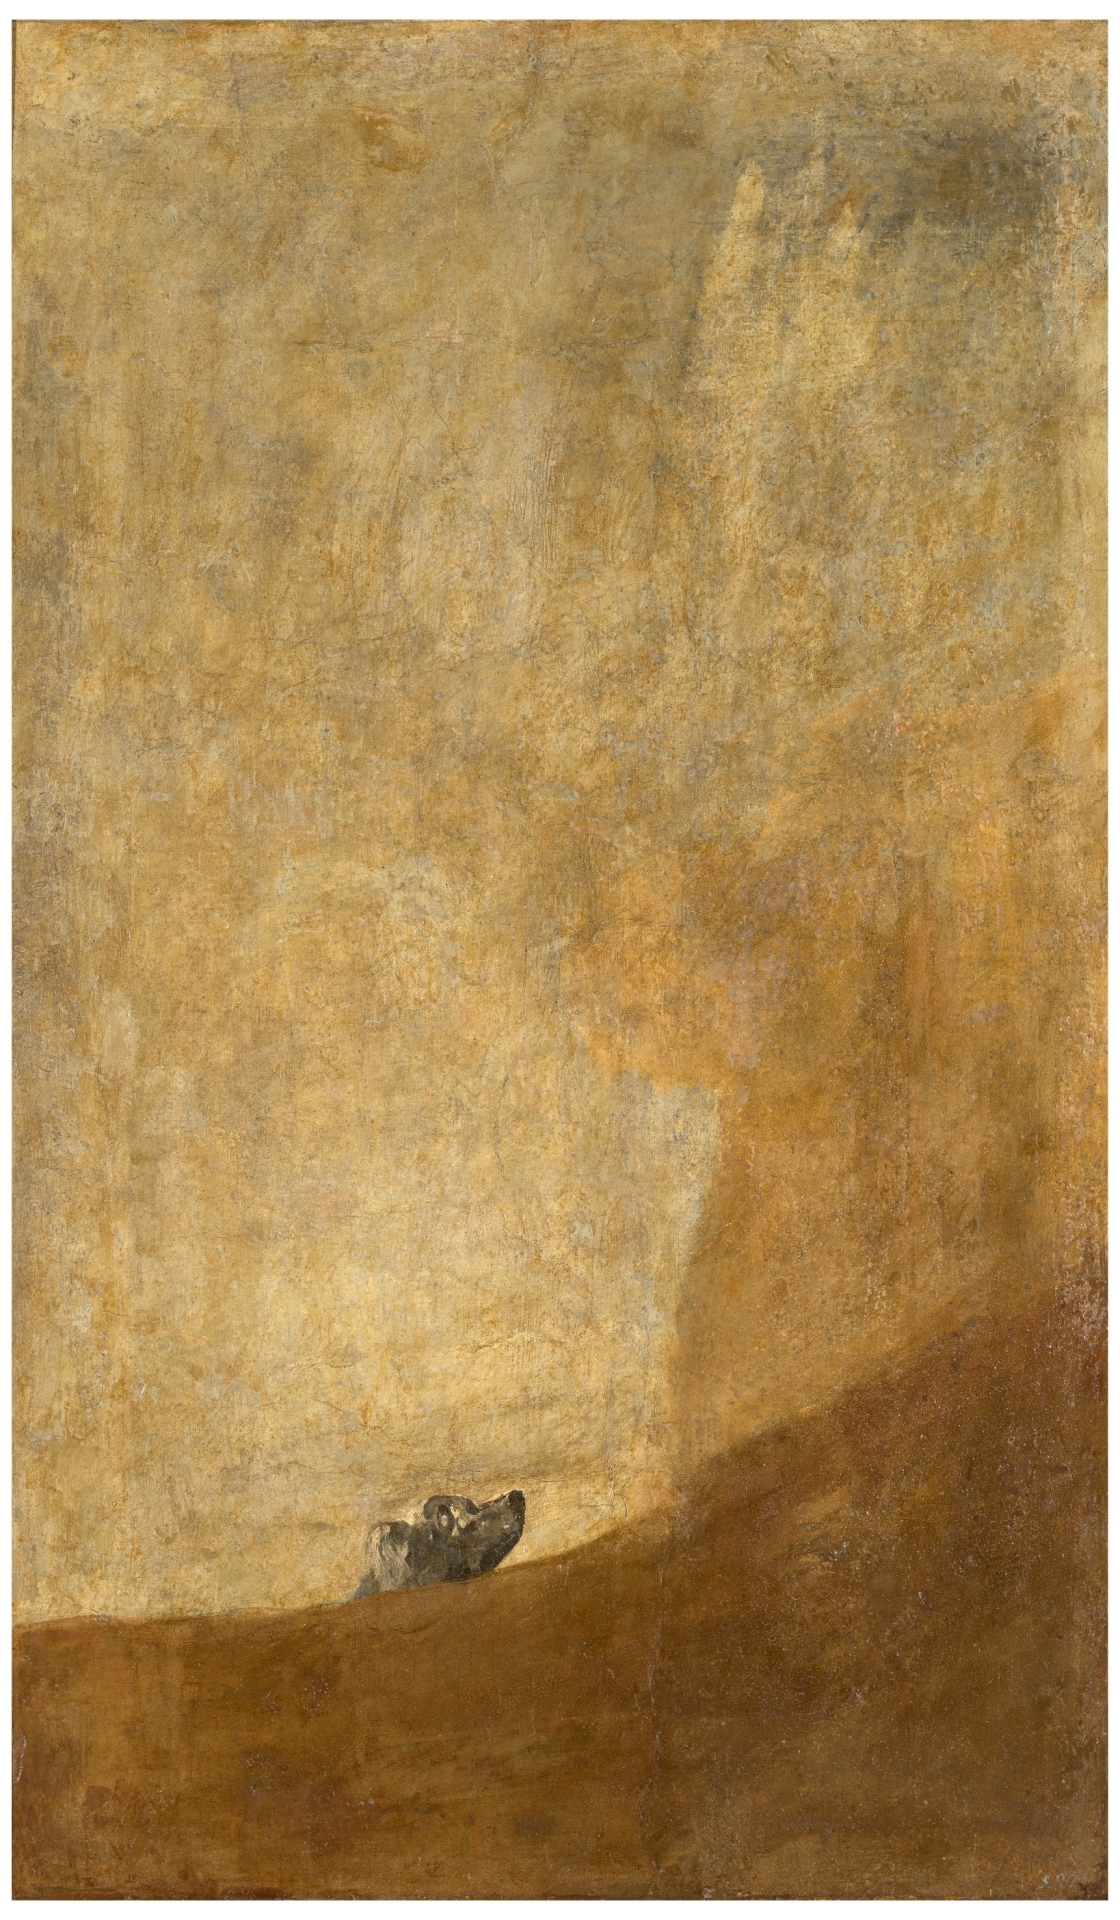
\includegraphics[width=0.8\textwidth]{perro.jpg}\hss}%
%% \end{minipage}
%% \begin{minipage}{0.5\textwidth}
%%   \Huge Preguntas
%% \end{minipage}
%% }
%% \end{frame}

\begin{frame}[fragile]
  \begin{center}
    {\Huge Tertulia}
    \vskip 1cm
    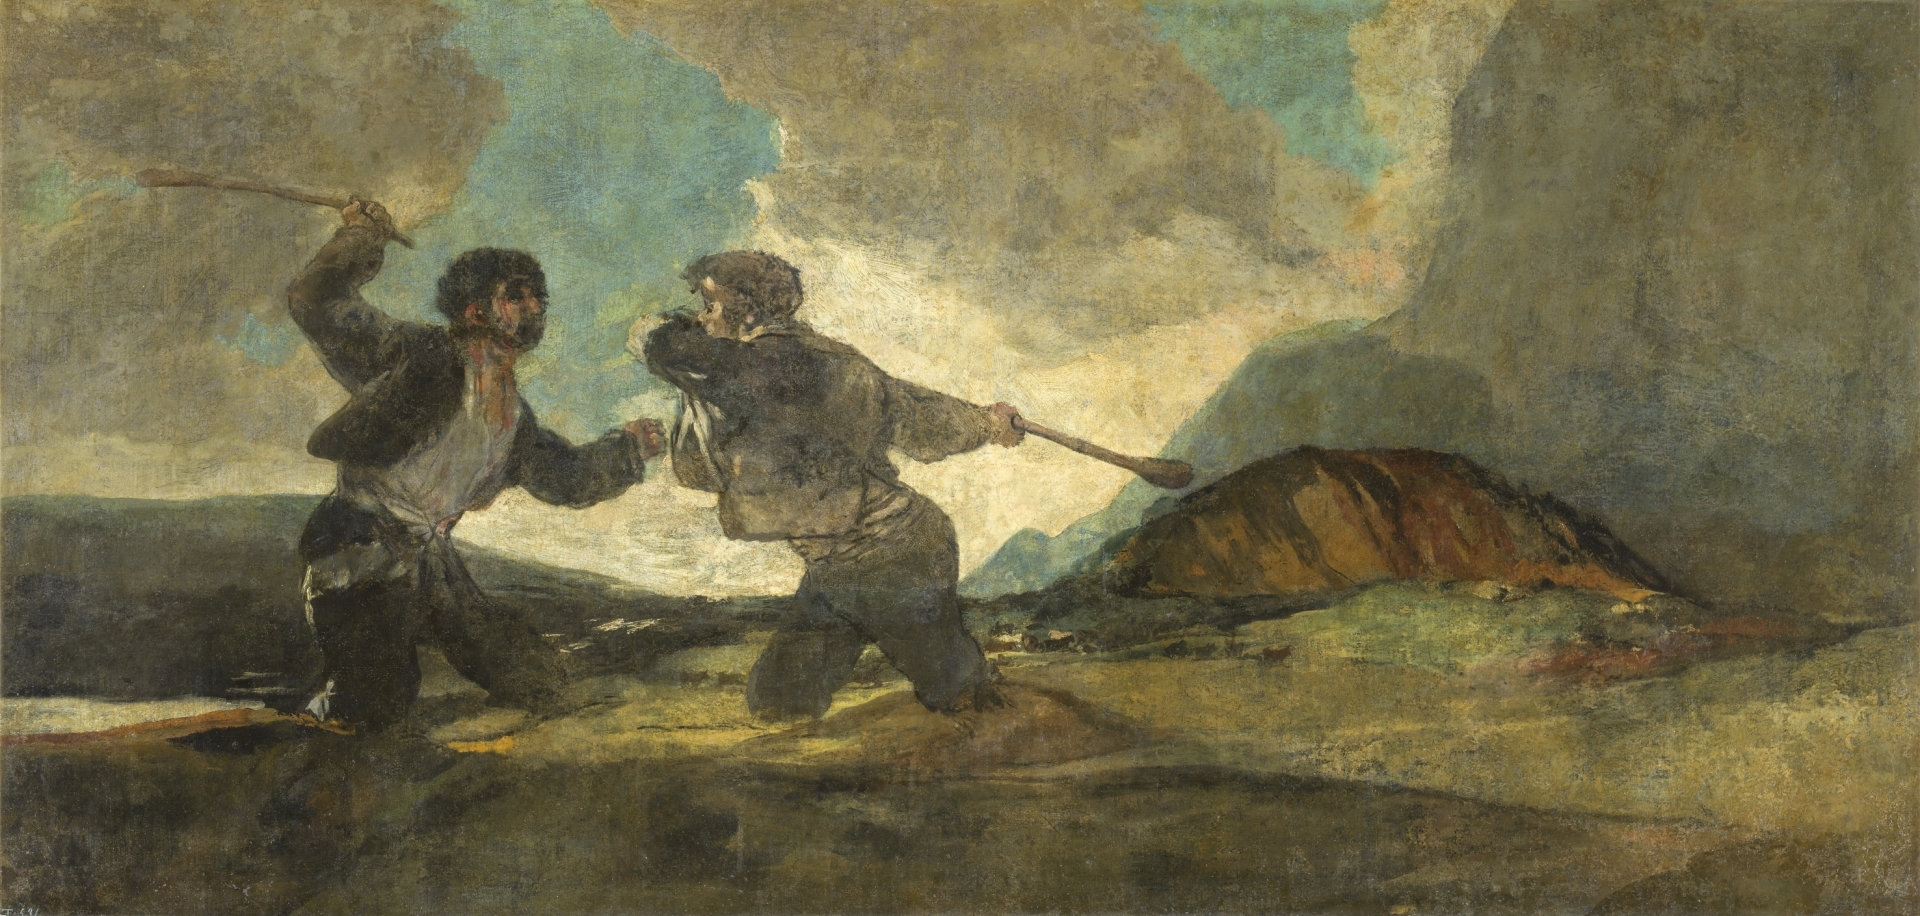
\includegraphics[width=0.8\textwidth]{duelo.jpg}
  \end{center}
\end{frame}


\end{document}
